\section{Примесь в двухуровневой модели}
Для гамильтониана \eqref{eff_so_ham} рассмотрим простейшую возможную примесь, а именно ---
потенциальную яму на одном из узлов решётки. В подходе сильной связи её гамильтониан ---
\begin{equation}
    V = \Delta E (a_{00}^\dagger a_{00} + b_{00}^\dagger b_{00})
\end{equation}
Уровни энергии \eqref{eff_so_ham} --- 
\begin{equation}
    E_p^2 = (\xi + \frac{1}{m}(2 - \cos{p_x} - \cos{p_y}))^2 + 4t^2(\sin^2{p_x} + \sin^2{p_y})
\end{equation}
Связанные состояния, как известно, даются уравнением на функцию Грина:
\begin{equation}    
    \det{\left[\mathbbm{1} - \Delta E \int \frac{d^2 p}{(2\pi)^2} 
            \frac{\omega + \hat{H}}{\omega^2 - E_p^2}\right]} = 1
\end{equation}
В последнем интеграле (от матрицы) недиагональные члены из--за симметрии обращаются в ноль.
Таким образом, связанные состояния сводятся к уравнениям
\begin{equation}
    \label{integrals}
    \left[
    \begin{split}
        &\int \frac{d^2 p}{(2\pi)^2} 
            \frac{\omega + \xi + \frac{1}{m}(2 - \cos{p_x} - \cos{p_y})}
                 {\omega^2 - E_p^2} = \frac{1}{\Delta E},\\
        &\int \frac{d^2 p}{(2\pi)^2} 
            \frac{-\omega + \xi + \frac{1}{m}(2 - \cos{p_x} - \cos{p_y})}
                 {\omega^2 - E_p^2} = -\frac{1}{\Delta E},
    \end{split}
    \right.
\end{equation}
Эти интегралы можно взять приближённо в круге небольшого радиуса $p_{\mathrm{max}}$,
если учесть, что при малых $p$ спектр близок к 
коническому. После интегрирования получается
\begin{equation}
    G(\omega,0,0)_{11} = -\frac{1}{8\pi}\frac{1}{m(4t^2 + \frac{\xi}{m})}
        \left[ p_{\mathrm{max}}^2 + 
            \left(2m(\omega+\xi) - \frac{\xi^2 - \omega^2}{4t^2 + \frac{\xi}{m}}\right) 
                \log{\left(1 + \frac{\left(4t^2 + \frac{\xi}{m}\right)p_{\mathrm{max}}^2}
                                    {\xi^2 - \omega^2}\right)}\right]
\end{equation}
Конечно, интегралы из \eqref{integrals} можно взять численно. Для 
$\xi, m, t = -0.03, 0.1, 0.5$ компоненты функции Грина изображены на графике.

\begin{figure}[h]
    \centering
    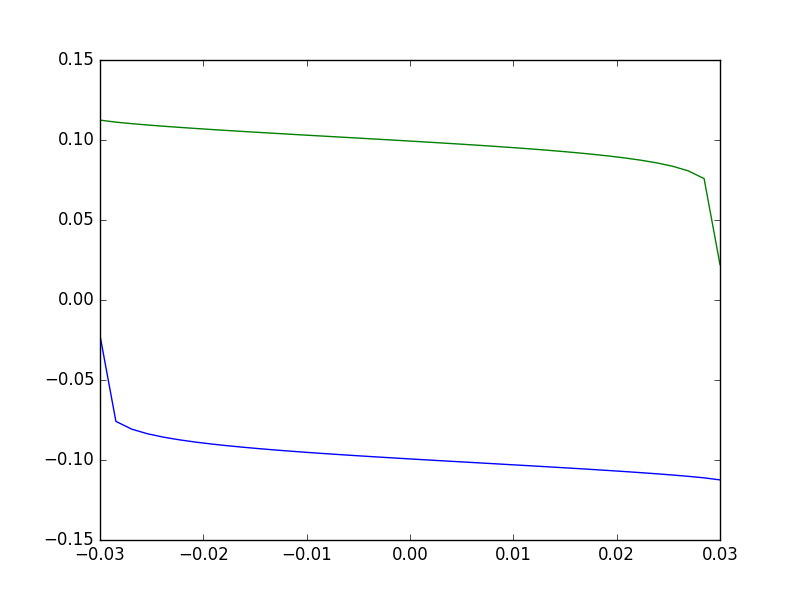
\includegraphics[width=0.8\linewidth]{green_functions.png}
    \caption{Компоненты функций Грина}
\end{figure}

Вычисление выше показывает, что происходит на краях этого графика. А именно, ``хвосты'' 
функций Грина растут логарифмически до бесконечности.
Таким образом, для малых $\Delta E < 0$ появляется одно связанное состояние около 
зоны проводимости. При дальнейшем росте возмущения появляется состояние около валентной зоны.
